% Partie 1.1 - l'IoT %

\subsection{L'IoT}

\textit{L'Internet of Things}, que nous appellerons IoT dans le reste de ce rapport, se traduit littéralement comme l'« Internet des objets », mais qu'est-ce-qu'un objet? Dans le monde de l'IoT les objets peuvent se référer à des biens (comme des meubles ou de l'électroménager), des machines, des véhicules, des immeubles ou bien même à quelque chose d'organique comme un être vivant (humain, animal ou plante) ou un sol (pour les cultures).

Alors la question est : Comment pouvons nous tout connecter ? En effet, comment faire en sorte qu'une plante possède un accès réseau ? C'est cela que l'IoT veut définir et représenter : une connectivité pour tout.

Mais d'abord que veut dire le mot connecter ? Prenons l'exemple d'une chaise, le fait qu'elle soit connectée veut dire que on peut avoir accès à de l'information la concernant, depuis n'importe où, grâce à un accès à Internet ; par exemple, est-elle occupée ? Si oui, qui est assis dessus ? Pour cela il faut donner certains attributs de cette chaise, comme un numéro d'identification unique, une manière de la distinguer d'un autre objet. 

Grâce à \textbf{IPv6}, il est désormais possible d’affecter une adresse unique à tout objet sans limite réelle, car l'espace adressable est sans limite pratique (mais il y a bien sur une limite physique). IPv4 est dépassé en terme de capacité d'adressage depuis longtemps mais grâce à des mécanismes comme le NAT/PAT, IPv4 est encore utilisé. Nous reviendrons sur IPv6 un peu plus tard dans ce rapport lors de notre présentation de 6LoWPAN.

Ensuite, nous avons besoins de donner à la chaise un moyen de communiquer avec le monde, soit de manière filaire soit sans fil, grâce à des antennes. D'où la nécessité des protocoles réseaux qui vont devoir transporter les informations ; malheureusement ceux que nous utilisons dans la vie tous les jours ne sont pas vraiment adaptés (IPv4, IPv6, Wi-Fi, etc.) à l'IoT, à cause de leur consommation électrique ou de leur bande-passante. C'est pourquoi de nouveaux protocoles ont vu le jour, spécialement adaptés à ces besoins. Certains se concentrent sur la puissance d'émission et d'autres sur la fiabilité dans les milieux bruités, mais tous prennent en compte certaines contraintes de l'IoT.

Nous parlons d'information et de données mais il faut bien les générer. Pour cela nous utilisons différents types de capteurs, par example un capteur de pression pour savoir si la chaise est occupée. Un autre type de capteur pourrait être une puce de localisation, voire un capteur d'identification qui pourra nous dire qui est assis sur la chaise et qui l'a été. De nos jours les capteurs sont extrêmement petits mais ont quand même certaines capacités comme de la mémoire, ce qui est très pratique en cas de coupure temporaire du réseaux ; en effet, les données ne sont pas forcément perdues.

\begin{figure}[H]
\centering
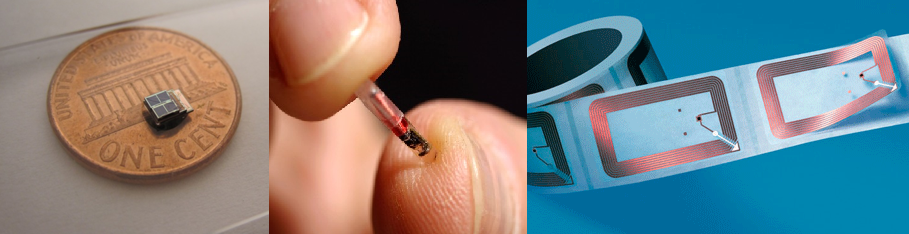
\includegraphics[width=15cm]{\rpDossier/images/capteurs.png}
\caption{Exemples de capteurs}
\label{sensors}
\end{figure}

Quelles seront les impacts et les possibilités de l'IoT ? Nous sommes limités seulement par notre imagination car nous changeons la façon de voir et de connecter les objets.

% Monitor %

Prenons quelques exemples pour montrer l'intérêt de l'IoT. Le \textit{monitoring} ne se résume pas qu’aux réseaux et aux machines, nous pouvons aussi l'appliquer pour surveiller l'état d'un patient en médecine. Imaginons quelqu'un avec un problème cardiaque, il possède un pacemaker qui est « connecté », cela veut dire qu'une application sur son téléphone peut dire à cette personne l'état de son cœur, mais aussi à son hôpital. Dans le cas d'une défaillance, une alerte est lancée à l'hôpital qui peut envoyer immédiatement une ambulance, en utilisant un tracker GPS intégré au tout pour localiser le patient.

Grâce à des algorithmes puissants, nous pourrons même prédire un problème potentiel sans que le patient vienne faire des visites de contrôles régulières, son pacemaker enverra les données pour lui. Avec le nombre de personnes agée de plus de 65 ans qui va doubler dans peu de temps, la e-santé et la télé-médecine vont devenir un des plus gros secteurs de l'IoT. 

% Search  %

Les tracas de quotidiens comme la perte de ses clefs ne seront plus un problème, en effet, dans le monde de l'IoT vos clés sont géo-localisables. Cela peut s'appliquer à plein de choses, si ce n'est à toutes, vous ne perdrez plus jamais rien.

% Manage %

Si nous savons où les choses sont et dans quels états elles sont, nous pouvons mieux les manager. Prenons le cas du trafic en ville : si nous savons où les voitures se situent et où elles vont, nous pouvons potentiellement éliminer les bouchons, optimiser les trajets et rediriger les flux plus facilement. Il en va de même pour l'énergie : si nous savons où l'énergie est requise, nous pouvons adapter la production et optimiser les coûts.

% Control %

L'IoT permet aussi de déléguer du contrôle : toujours dans une optique d'optimisation énergétique, nous pouvons déléguer l'heure de départ d'une machine à laver, d'un lave-vaisselle à un contrôleur distant qui lancera le programme au moment où l'énergie sera la moins chère.

% RV + IoT %

Un autre marché que l'IoT va investir est la réalité augmentée (en particulier les jeux vidéo). En effet, en utilisant la réalité augmentée, nous pouvons superposer la réalité (filmée par une caméra) et le monde virtuel grâce à un traitement logiciel. L'IoT va simplement étendre le panel de fonctionnalités de manière infinie en permettant d'interagir avec l'environnement. Par example, il suffirait de lancer son application de réalité augmentée et de toucher l'objet avec lequel nous voulons interagir pour se voir proposer des actions. Le panel d'actions se limite seulement à ce que le développeur veut laisser les gens faire.

\begin{figure}[H]
\centering
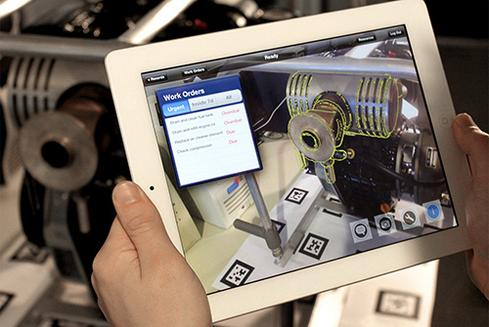
\includegraphics[width=10cm]{\rpDossier/images/ariot.jpg}
\caption{Réalité augmentée associée à l’IoT}
\label{ariot}
\end{figure}

% Privacy %

Le fait est qu'avec l'IoT, la notion de « privé » devient très floue. Nous tenons à évoquer ce point car l'IoT va quelque peu bousculer certaines habitudes. Reprenons notre chaise, comme dit précédemment, nous pouvons facilement savoir qui était assis dessus grâce à notre identifiant unique. Les risques liés à la protection de notre vie privée augmentent avec l'IoT, qui collecte agrège des bouts de données liées aux services que l'appareil propose. Le recoupement d'informations peut assez vite convertir des données banales en données personnelles car les événements (actions de l'utilisateur) possèdent un lieu, une heure, une récurrence, etc. L'achat régulier de différents types de nourriture peut révéler la religion ou des problèmes de santé. C'est un véritable enjeu lié au \emph{Big Data} que l'exploitation des données générées par l'IoT. Le volume de données va pouvoir permettre aux exploitants de convertir ces données « publiques » en données « privées ».

% Security %

Maintenant, il faut aussi se placer du côté de l'exploitant qui va vouloir protéger ses informations ; c'est pour cela que la sécurisation des transmissions est l'un des enjeux essentiels de l'IoT. L'inconvénient est que la plupart du temps, les capteurs n'ont aucune puissance de calcul pour chiffrer l'information, actuellement les capteurs se concentrent plus sur l'intégrité du message et à établir une connexion sécurisée \todo[que sur la sécurisation des connexions ?]. Plus la technologie évoluera, plus la sécurité de l'information se rapprochera de l'appareil, pour ultimement devenir embarquée. 

Il est vrai qu'un simple \textit{sniffer} réglé sur la bonne fréquence permettra d’intercepter les informations si celles-ci sont transmisses sur un canal sans fil. En effet sans chiffrement, elles sont envoyées en clair. Cela ne pose pas trop de problème pour des données non-confidentielles mais peut vite devenir problématique si les informations recueillies sont de nature plus sensibles.

% Data Processing % 

Nous avons parlé précédemment de traitement de l'information, mais au vu des volumes de données générées, ce n'est pas sur un simple PC de bureau que nous pourrons analyser les données. Avec vingt milliards d'objets connectés en 2020, les datacenters feront face à des charges de travail inédites. Le volume de données traitées n'aura jamais était aussi important et ne fera que grossir aux fil des années. Les fournisseurs commencent dès aujourd'hui à concevoir leur datacenters en prévision de l'IoT qui arrive à grand pas.

Mais revenons à un niveau plus bas, celui de la transmission entre les capteurs. Nous ne sommes pas encore sur les infrastructures des FAI mais dans notre réseau local. Ce même réseau est celui qui est le plus proche de l'utilisateur. 
